\numoptstrue
\yearpaper{2017}{7 May 2017 \textperiodcentered{} Test Booklet Code B \textperiodcentered{} Physics Q 136--180 \textperiodcentered{} 180 Marks}{In this paper Physics is the last section; the original question numbers are kept.}
\setcounter{qno}{135}
\begin{multicols}{2}

\QQ{Two astronauts are floating in gravitational free space after having lost contact with their spaceship. The two will:}
{\opt{move towards each other.}{move away from each other.}{will become stationary.}{keep floating at the same distance between them.}}

\QQ{Young's double slit experiment is first performed in air and then in a medium other than air. It is found that $8^{\text{th}}$ bright fringe in the medium lies where $5^{\text{th}}$ dark fringe lies in air. The refractive index of the medium is nearly:}
{\opt{1.59}{1.69}{1.78}{1.25}}

\QQ{In a common emitter transistor amplifier the audio signal voltage across the collector is 3\,V. The resistance of collector is $3\unit{k\Omega}$. If current gain is 100 and the base resistance is $2\unit{k\Omega}$, the voltage and power gain of the amplifier is:}
{\opt{15 and 200}{150 and 15000}{20 and 2000}{200 and 1000}}

\QQ{An arrangement of three parallel straight wires placed perpendicular to plane of paper carrying same current `$I$' along the same direction is shown in Fig. Magnitude of force per unit length on the middle wire `B' is given by:
\fig{\begin{tikzpicture}[scale=0.8]
\draw (0,1.5) circle (0.12) node[above left,lbl]{B}; \fill (0,1.5) circle (0.04); \draw (1.6,1.5) circle (0.12) node[right=2pt,lbl]{C}; \fill (1.6,1.5) circle (0.04); \draw (0,0) circle (0.12) node[left=2pt,lbl]{A}; \fill (0,0) circle (0.04);
\draw (0.12,1.5) -- (1.48,1.5) node[midway,above,lbl]{$d$}; \draw (0,1.38) -- (0,0.12) node[midway,left,lbl]{$d$}; \draw (0,1.2) -- (0.3,1.2) -- (0.3,1.5); \node[lbl] at (0.55,1.15) {$90^\circ$};
\end{tikzpicture}}}
{\opt{$\dfrac{2\mu_0i^2}{\pi d}$}{$\dfrac{\sqrt2\mu_0i^2}{\pi d}$}{$\dfrac{\mu_0i^2}{\sqrt2\pi d}$}{$\dfrac{\mu_0i^2}{2\pi d}$}}

\QQ{The de-Broglie wavelength of a neutron in thermal equilibrium with heavy water at a temperature $T$ (Kelvin) and mass $m$, is:}
{\opt{$\dfrac h{\sqrt{3mkT}}$}{$\dfrac{2h}{\sqrt{3mkT}}$}{$\dfrac{2h}{\sqrt{mkT}}$}{$\dfrac h{\sqrt{mkT}}$}}

\QQ{Radioactive material `A' has decay constant `$8\lambda$' and material `B' has decay constant `$\lambda$'. Initially they have same number of nuclei. After what time, the ratio of number of nuclei of material `B' to that `A' will be $\dfrac1e$?}
{\opt{$\dfrac1{7\lambda}$}{$\dfrac1{8\lambda}$}{$\dfrac1{9\lambda}$}{$\dfrac1\lambda$}}

\QQ{The given electrical network is equivalent to:
\fig{\begin{circuitikz}[scale=0.7,transform shape]
\draw (0,0) node[nor port](G1){}; \draw (2.6,0) node[nor port](G2){}; \draw (4.6,0) node[not port](N){};
\draw (G1.in 1) -- ++(-0.4,0) node[circ]{} node[left]{A}; \draw (G1.in 2) -- ++(-0.4,0) node[circ]{} node[left]{B};
\draw (G1.out) -- ++(0.3,0) coordinate(m); \draw (m) |- (G2.in 1); \draw (m) |- (G2.in 2); \draw (G2.out) -- (N.in); \draw (N.out) -- ++(0.3,0) node[circ]{} node[above]{Y};
\end{circuitikz}}}
{\opt{OR gate}{NOR gate}{NOT gate}{AND gate}}

\QQ{The resistance of a wire is `$R$' ohm. If it is melted and stretched to `$n$' times its original length, its new resistance will be:}
{\opt{$\dfrac Rn$}{$n^2R$}{$\dfrac R{n^2}$}{$nR$}}

\QQ{Two cars moving in opposite directions approach each other with speed of $22\unit{m/s}$ and $16.5\unit{m/s}$ respectively. The driver of the first car blows a horn having a frequency 400\,Hz. The frequency heard by the driver of the second car is [velocity of sound $340\unit{m/s}$]:}
{\opt{361\,Hz}{411\,Hz}{448\,Hz}{350\,Hz}}

\QQ{In an electromagnetic wave in free space the root mean square value of the electric field is $E_{\text{rms}} = 6\unit{V/m}$. The peak value of the magnetic field is:}
{\opt{$2.83\times10^{-8}\unit{T}$}{$0.70\times10^{-8}\unit{T}$}{$4.23\times10^{-8}\unit{T}$}{$1.41\times10^{-8}\unit{T}$}}

\QQ{Two rods A and B of different materials are welded together as shown in figure. Their thermal conductivities are $K_1$ and $K_2$. The thermal conductivity of the composite rod will be:
\fig{\begin{tikzpicture}[scale=0.8]
\fill[pattern=north east lines] (0,0.5) rectangle (2.6,1); \fill[pattern=north west lines] (0,0) rectangle (2.6,0.5); \draw (0,0) rectangle (2.6,1); \draw (0,0.5) -- (2.6,0.5);
\node[lbl,fill=white,inner sep=1pt] at (1.3,0.75) {A\quad $K_1$}; \node[lbl,fill=white,inner sep=1pt] at (1.3,0.25) {B\quad $K_2$};
\node[lbl,left] at (0,0.5) {$T_1$}; \node[lbl,right] at (2.6,0.5) {$T_2$}; \draw[<->] (0,-0.25) -- (2.6,-0.25) node[midway,below,lbl]{$d$};
\end{tikzpicture}}}
{\opt{$\dfrac{3(K_1+K_2)}2$}{$K_1+K_2$}{$2(K_1+K_2)$}{$\dfrac{K_1+K_2}2$}}

\QQ{Which one of the following represents forward bias diode?}
{\opt{$-4$\,V\,\begin{circuitikz}[scale=0.5,transform shape,baseline=-2pt]\draw (0,0) to[empty diode] (1.5,0) to[R] (3,0);\end{circuitikz}\,$-3$\,V}{$-2$\,V\,\begin{circuitikz}[scale=0.5,transform shape,baseline=-2pt]\draw (0,0) to[empty diode] (1.5,0) to[R] (3,0);\end{circuitikz}\,$+2$\,V}{3\,V\,\begin{circuitikz}[scale=0.5,transform shape,baseline=-2pt]\draw (0,0) to[empty diode] (1.5,0) to[R] (3,0);\end{circuitikz}\,5\,V}{0\,V\,\begin{circuitikz}[scale=0.5,transform shape,baseline=-2pt]\draw (0,0) to[empty diode] (1.5,0) to[R] (3,0);\end{circuitikz}\,$-2$\,V}}

\QQ{A 250-turn rectangular coil of length $2.1\unit{cm}$ and width $1.25\unit{cm}$ carries a current of $85\unit{\mu A}$ and subjected to a magnetic field of strength $0.85\unit{T}$. Work done for rotating the coil by $180^\circ$ against the torque is:}
{\opt{$4.55\unit{\mu J}$}{$2.3\unit{\mu J}$}{$1.15\unit{\mu J}$}{$9.1\unit{\mu J}$}}

\QQ{If $\theta_1$ and $\theta_2$ be the apparent angles of dip observed in two vertical planes at right angles to each other, then the true angle of dip $\theta$ is given by:}
{\opt{$\tan^2\theta = \tan^2\theta_1+\tan^2\theta_2$}{$\cot^2\theta = \cot^2\theta_1-\cot^2\theta_2$}{$\tan^2\theta = \tan^2\theta_1-\tan^2\theta_2$}{$\cot^2\theta = \cot^2\theta_1+\cot^2\theta_2$}}

\QQ{A potentiometer is an accurate and versatile device to make electrical measurements of E.M.F.\ because the method involves:}
{\opt{potential gradients}{a condition of no current flow through the galvanometer}{a combination of cells, galvanometer and resistances}{cells}}

\QQ{The ratio of resolving powers of an optical microscope for two wavelengths $\lambda_1 = 4000\unit{\text{\AA}}$ and $\lambda_2 = 6000\unit{\text{\AA}}$ is:}
{\opt{9:4}{3:2}{16:81}{8:27}}

\QQ{A thin prism having refracting angle $10^\circ$ is made of glass of refractive index 1.42. This prism is combined with another thin prism of glass of refractive index 1.7. This combination produces dispersion without deviation. The refracting angle of second prism should be:}
{\opt{$6^\circ$}{$8^\circ$}{$10^\circ$}{$4^\circ$}}

\QQ{A capacitor is charged by a battery. The battery is removed and another identical uncharged capacitor is connected in parallel. The total electrostatic energy of resulting system:}
{\opt{decreases by a factor of 2}{remains the same}{increases by a factor of 2}{increases by a factor of 4}}

\QQ{Preeti reached the metro station and found that the escalator was not working. She walked up the stationary escalator in time $t_1$. On other days, if she remains stationary on the moving escalator, then the escalator takes her up in time $t_2$. The time taken by her to walk up on the moving escalator will be:}
{\opt{$\dfrac{t_1t_2}{t_2-t_1}$}{$\dfrac{t_1t_2}{t_2+t_1}$}{$t_1-t_2$}{$\dfrac{t_1+t_2}2$}}

\QQ{Thermodynamic processes are indicated in the following diagram.
\fig{\begin{tikzpicture}[scale=1.15]
\draw[->] (0,0) -- (3.6,0) node[right,lbl]{$V$}; \draw[->] (0,0) -- (0,2.6) node[above,lbl]{$P$};
\draw (0.3,2.2) .. controls (0.8,1.0) and (1.8,0.6) .. (2.8,0.45) node[right,lbl]{300\,K}; \draw (0.6,2.3) .. controls (1.1,1.3) and (2.0,0.9) .. (2.9,0.75) node[right,lbl]{500\,K}; \draw (0.9,2.4) .. controls (1.5,1.5) and (2.3,1.2) .. (3.0,1.1) node[right,lbl]{700\,K};
\coordinate (i) at (1.0,1.6); \fill (i) circle (1.2pt) node[above left,lbl]{$i$};
\draw[->] (i) -- (1.0,0.85) node[left,lbl]{f}; \node[lbl] at (0.85,1.25) {I}; \draw[->] (i) -- (1.5,1.0) node[right,lbl]{f}; \node[lbl] at (1.35,1.35) {II};
\draw[->] (i) -- (1.7,1.6) node[right,lbl]{f}; \node[lbl] at (1.45,1.8) {IV}; \draw[->] (i) -- (1.7,1.25); \node[lbl] at (1.9,1.35) {III};
\end{tikzpicture}}
Match the following:\par\smallskip
\begin{tabular}{@{}ll@{\qquad}ll@{}}
P. & Process I & a. & Adiabatic\\ Q. & Process II & b. & Isobaric\\ R. & Process III & c. & Isochoric\\ S. & Process IV & d. & Isothermal
\end{tabular}}
{\opt{P$\to$c, Q$\to$a, R$\to$d, S$\to$b}{P$\to$c, Q$\to$d, R$\to$b, S$\to$a}{P$\to$d, Q$\to$b, R$\to$a, S$\to$c}{P$\to$a, Q$\to$c, R$\to$d, S$\to$b}}

\QQ{One end of string of length $l$ is connected to a particle of mass `$m$' and the other end is connected to a small peg on a smooth horizontal table. If the particle moves in circle with speed `$v$', the net force on the particle (directed towards center) will be ($T$ represents the tension in the string):}
{\opt{$T+\dfrac{mv^2}l$}{$T-\dfrac{mv^2}l$}{Zero}{$T$}}

\QQ{The two nearest harmonics of a tube closed at one end and open at other end are 220\,Hz and 260\,Hz. What is the fundamental frequency of the system?}
{\opt{20\,Hz}{30\,Hz}{40\,Hz}{10\,Hz}}

\QQ{The photoelectric threshold wavelength of silver is $3250\times10^{-10}\unit{m}$. The velocity of the electron ejected from a silver surface by ultraviolet light of wavelength $2536\times10^{-10}\unit{m}$ is: (Given $h = 4.14\times10^{-15}\unit{eV\,s}$ and $c = 3\times10^8\unit{m\,s^{-1}}$)}
{\opt{$\approx0.6\times10^6\unit{m\,s^{-1}}$}{$\approx61\times10^3\unit{m\,s^{-1}}$}{$\approx0.3\times10^6\unit{m\,s^{-1}}$}{$\approx6\times10^5\unit{m\,s^{-1}}$}}

\QQ{Figure shows a circuit that contains three identical resistors with resistance $R = 9.0\unit{\Omega}$ each, two identical inductors with inductance $L = 2.0\unit{mH}$ each, and an ideal battery with emf $\varepsilon = 18\unit{V}$. The current `$i$' through the battery just after the switch closed is,
\fig{\begin{circuitikz}[scale=0.55,transform shape,font=\Large]
\draw (0,0) to[battery1,l=$\varepsilon$,invert] (0,3) -- (6,3);
\draw (2,3) to[L,l_=L] (2,1.5) to[R,l_=R] (2,0); \draw (4,3) to[R,l=R] (4,0); \draw (6,3) to[R,l=R] (6,1.5) to[L,l_=L] (6,0);
\draw (6,1.5) -- (7.5,1.5) to[C,l=C] (7.5,0) -- (6,0);
\draw (0,0) to[nos] (2,0) -- (6,0);
\end{circuitikz}}}
{\opt{0.2\,A}{2\,A}{0 ampere}{2\,mA}}

\QQ{A spherical black body with a radius of $12\unit{cm}$ radiates 450 watt power at 500\,K. If the radius were halved and the temperature doubled, the power radiated in watt would be:}
{\opt{450}{1000}{1800}{225}}

\QQ{A rope is wound around a hollow cylinder of mass $3\unit{kg}$ and radius $40\unit{cm}$. What is the angular acceleration of the cylinder if the rope is pulled with a force of $30\unit{N}$?}
{\opt{$0.25\unit{rad/s^2}$}{$25\unit{rad/s^2}$}{$5\unit{m/s^2}$}{$25\unit{m/s^2}$}}

\QQ{Two discs of same moment of inertia rotating about their regular axis passing through centre and perpendicular to the plane of disc with angular velocities $\omega_1$ and $\omega_2$. They are brought into contact face to face coinciding the axis of rotation. The expression for loss of energy during this process is:}
{\opt{$\dfrac14I(\omega_1-\omega_2)^2$}{$I(\omega_1-\omega_2)^2$}{$\dfrac18(\omega_1-\omega_2)^2$}{$\dfrac12I(\omega_1+\omega_2)^2$}}

\QQ{A gas mixture consists of 2 moles of $\mathrm O_2$ and 4 moles of Ar at temperature $T$. Neglecting all vibrational modes, the total internal energy of the system is:}
{\opt{$15RT$}{$9RT$}{$11RT$}{$4RT$}}

\QQ{The bulk modulus of a spherical object is `$B$'. If it is subjected to uniform pressure `$p$', the fractional decrease in radius is:}
{\opt{$\dfrac B{3p}$}{$\dfrac{3p}B$}{$\dfrac p{3B}$}{$\dfrac pB$}}

\QQ{Which of the following statements are correct?
\begin{stmts}[(\alph*)]
\item Centre of mass of a body always coincides with the centre of gravity of the body.
\item Centre of mass of a body is the point at which the total gravitational torque on the body is zero.
\item A couple on a body produce both translational and rotational motion in a body.
\item Mechanical advantage greater than one means that small effort can be used to lift a large load.
\end{stmts}}
{\opt{(a) and (b)}{(b) and (c)}{(c) and (d)}{(b) and (d)}}

\QQ{The acceleration due to gravity at a height 1\,km above the earth is the same as at a depth $d$ below the surface of earth. Then:}
{\opt{$d = 1\unit{km}$}{$d = \dfrac32\unit{km}$}{$d = 2\unit{km}$}{$d = \dfrac12\unit{km}$}}

\QQ{Two blocks A and B of masses $3m$ and $m$ respectively are connected by a massless and inextensible string. The whole system is suspended by a massless spring as shown in figure. The magnitudes of acceleration of A and B immediately after the string is cut, are respectively:
\fig{\begin{tikzpicture}[scale=0.7]
\fill[pattern=north east lines] (-0.7,2.6) rectangle (0.7,2.8); \draw (-0.7,2.6) -- (0.7,2.6);
\draw[decorate,decoration={coil,aspect=0.5,segment length=3pt,amplitude=4pt}] (0,2.6) -- (0,1.4);
\draw (-0.4,1.0) rectangle (0.4,1.4) node[midway,lbl]{A}; \node[lbl,right] at (0.4,1.2) {$3m$}; \draw (0,1.0) -- (0,0.4);
\draw (-0.3,0) rectangle (0.3,0.4) node[midway,lbl]{B}; \node[lbl,right] at (0.3,0.2) {$m$};
\end{tikzpicture}}}
{\opt{$\dfrac g3$, $g$}{$g$, $g$}{$\dfrac g3$, $\dfrac g3$}{$g$, $\dfrac g3$}}

\QQ{The ratio of wavelengths of the last line of Balmer series and the last line of Lyman series is:}
{\opt{1}{4}{0.5}{2}}

\QQ{A beam of light from a source L is incident normally on a plane mirror fixed at a certain distance $x$ from the source. The beam is reflected back as a spot on a scale placed just above the source L. When the mirror is rotated through a small angle $\theta$, the spot of the light is found to move through a distance $y$ on the scale. The angle $\theta$ is given by:}
{\opt{$\dfrac yx$}{$\dfrac x{2y}$}{$\dfrac xy$}{$\dfrac y{2x}$}}

\QQ{A spring of force constant $k$ is cut into lengths of ratio 1:2:3. They are connected in series and the new force constant is $k'$. Then they are connected in parallel and force constant is $k''$. Then $k':k''$ is:}
{\opt{1:9}{1:11}{1:14}{1:6}}

\QQ{The diagrams below show regions of equipotentials.
\fig{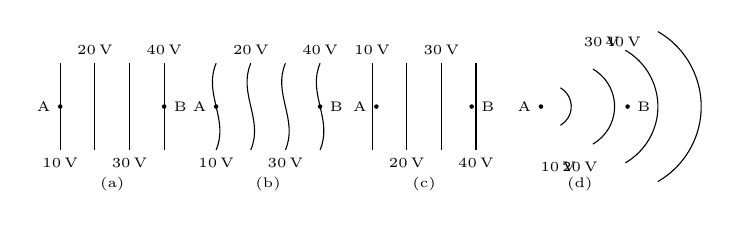
\begin{tikzpicture}[scale=0.55]
\foreach \x/\v in {0/10,0.8/20,1.6/30,2.4/40} {\draw (\x,0) -- (\x,2); \node[font=\tiny] at (\x,{mod(\x*10,16)<1?-0.3:2.3}) {\v\,V};}
\fill (0,1) circle (1.5pt) node[left,font=\tiny]{A}; \fill (2.4,1) circle (1.5pt) node[right,font=\tiny]{B}; \node[font=\tiny] at (1.2,-0.8) {(a)};
\begin{scope}[xshift=3.6cm]
\foreach \x/\v in {0/10,0.8/20,1.6/30,2.4/40} {\draw (\x,0) .. controls (\x+0.3,0.7) and (\x-0.3,1.3) .. (\x,2); \node[font=\tiny] at (\x,{mod(\x*10,16)<1?-0.3:2.3}) {\v\,V};}
\fill (0,1) circle (1.5pt) node[left,font=\tiny]{A}; \fill (2.4,1) circle (1.5pt) node[right,font=\tiny]{B}; \node[font=\tiny] at (1.2,-0.8) {(b)};
\end{scope}
\begin{scope}[xshift=7.2cm]
\foreach \x/\v in {0/10,0.8/20,1.6/30,2.4/40} {\draw (\x,0) -- (\x,2); \node[font=\tiny] at (\x,{mod(\x*10,16)<1?2.3:-0.3}) {\v\,V};}
\fill (0.1,1) circle (1.5pt) node[left,font=\tiny]{A}; \fill (2.3,1) circle (1.5pt) node[right,font=\tiny]{B}; \node[font=\tiny] at (1.2,-0.8) {(c)};
\end{scope}
\begin{scope}[xshift=10.8cm]
\foreach \r/\v in {0.5/10,1.0/20,1.5/30,2.0/40} {\draw (\r,1) ++(60:\r) arc (60:-60:\r); \node[font=\tiny] at (\r+0.2,{\r>1.2?2.5:-0.4}) {\v\,V};}
\fill (0.3,1) circle (1.5pt) node[left,font=\tiny]{A}; \fill (2.3,1) circle (1.5pt) node[right,font=\tiny]{B}; \node[font=\tiny] at (1.2,-0.8) {(d)};
\end{scope}
\end{tikzpicture}}
A positive charge is moved from A to B in each diagram.}
{\opt{In all the four cases the work done is the same.}{Minimum work is required to move $q$ in figure (a).}{Maximum work is required to move $q$ in figure (b).}{Maximum work is required to move $q$ in figure (c).}}

\QQ{Suppose the charge of a proton and an electron differ slightly. One of them is $-e$, the other is $(e+\Delta e)$. If the net of electrostatic force and gravitational force between two hydrogen atoms placed at a distance $d$ (much greater than atomic size) apart is zero, then $\Delta e$ is of the order of [Given mass of hydrogen $m_h = 1.67\times10^{-27}\unit{kg}$]}
{\opt{$10^{-23}\unit{C}$}{$10^{-37}\unit{C}$}{$10^{-47}\unit{C}$}{$10^{-20}\unit{C}$}}

\QQ{A physical quantity of the dimensions of length that can be formed out of $c$, $G$ and $\dfrac{e^2}{4\pi\varepsilon_0}$ is [$c$ is velocity of light, $G$ is universal constant of gravitation and $e$ is charge]:}
{\opt{$c^2\left[G\dfrac{e^2}{4\pi\varepsilon_0}\right]^{1/2}$}{$\dfrac1{c^2}\left[\dfrac{e^2}{G4\pi\varepsilon_0}\right]^{1/2}$}{$\dfrac1cG\dfrac{e^2}{4\pi\varepsilon_0}$}{$\dfrac1{c^2}\left[G\dfrac{e^2}{4\pi\varepsilon_0}\right]^{1/2}$}}

\QQ{Two Polaroids $P_1$ and $P_2$ are placed with their axis perpendicular to each other. Unpolarised light $I_0$ is incident on $P_1$. A third polaroid $P_3$ is kept in between $P_1$ and $P_2$ such that its axis makes an angle $45^\circ$ with that of $P_1$. The intensity of transmitted light through $P_2$ is:}
{\opt{$\dfrac{I_0}4$}{$\dfrac{I_0}8$}{$\dfrac{I_0}{16}$}{$\dfrac{I_0}2$}}

\QQ{A particle executes linear simple harmonic motion with an amplitude of $3\unit{cm}$. When the particle is at $2\unit{cm}$ from the mean position, the magnitude of its velocity is equal to that of its acceleration. Then its time period in seconds is:}
{\opt{$\dfrac{\sqrt5}{2\pi}$}{$\dfrac{4\pi}{\sqrt5}$}{$\dfrac{2\pi}{\sqrt3}$}{$\dfrac{\sqrt5}\pi$}}

\QQ{A U tube with both ends open to the atmosphere, is partially filled with water. Oil, which is immiscible with water, is poured into one side until it stands at a distance of $10\unit{mm}$ above the water level on the other side. Meanwhile the water rises by $65\unit{mm}$ from its original level (see diagram). The density of the oil is:
\fig{\begin{tikzpicture}[scale=0.55]
\draw (0,4) -- (0,1) arc (180:360:1) -- (2,4); \draw (0.5,4) -- (0.5,1) arc (180:360:0.5) -- (1.5,4);
\fill[pattern=dots] (0,1.2) rectangle (0.5,3.7); \node[lbl,above] at (0.25,4) {$P_a$}; \node[lbl,above] at (1.75,4) {$P_a$};
\draw[densely dotted] (-0.3,3.7) node[left,lbl]{A} -- (2.6,3.7) node[right,lbl]{F}; \draw[densely dotted] (0.5,3.3) -- (2.6,3.3) node[right,lbl]{E (final water level)};
\draw[densely dotted] (0.5,2.25) -- (2.6,2.25) node[right,lbl]{D (initial water level)}; \draw[densely dotted] (-0.3,1.2) node[left,lbl]{B} -- (2.6,1.2) node[right,lbl]{C};
\draw[<->] (1.0,2.25) -- (1.0,3.3) node[midway,fill=white,inner sep=0.5pt,font=\tiny]{65\,mm}; \draw[<->] (1.0,1.2) -- (1.0,2.25) node[midway,fill=white,inner sep=0.5pt,font=\tiny]{65\,mm};
\node[lbl,left] at (-0.1,2.5) {Oil}; \node[lbl] at (2.5,0.2) {Water}; \node[font=\tiny] at (3.1,3.5) {10\,mm};
\end{tikzpicture}}}
{\opt{$425\unit{kg\,m^{-3}}$}{$800\unit{kg\,m^{-3}}$}{$928\unit{kg\,m^{-3}}$}{$650\unit{kg\,m^{-3}}$}}

\QQ{Consider a drop of rain water having mass 1\,g falling from a height of 1\,km. It hits the ground with a speed of $50\unit{m/s}$. Take `$g$' constant with a value $10\unit{m/s^2}$. The work done by the (i) gravitational force and the (ii) resistive force of air is:}
{\opt{(i) 1.25\,J (ii) $-8.25$\,J}{(i) 100\,J (ii) 8.75\,J}{(i) 10\,J (ii) $-8.75$\,J}{(i) $-10$\,J (ii) $-8.25$\,J}}

\QQ{The $x$ and $y$ coordinates of the particle at any time are $x = 5t-2t^2$ and $y = 10t$ respectively, where $x$ and $y$ are in meters and $t$ in seconds. The acceleration of the particle at $t = 2\unit{s}$ is:}
{\opt{$5\unit{m/s^2}$}{$-4\unit{m/s^2}$}{$-8\unit{m/s^2}$}{0}}

\QQ{A long solenoid of diameter $0.1\unit{m}$ has $2\times10^4$ turns per meter. At the centre of the solenoid, a coil of 100 turns and radius $0.01\unit{m}$ is placed with its axis coinciding with the solenoid axis. The current in the solenoid reduces at a constant rate to 0\,A from 4\,A in $0.05\unit{s}$. If the resistance of the coil is $10\pi^2\unit{\Omega}$, the total charge flowing through the coil during this time is:}
{\opt{$16\unit{\mu C}$}{$32\unit{\mu C}$}{$16\pi\unit{\mu C}$}{$32\pi\unit{\mu C}$}}

\QQ{A carnot engine having an efficiency of $\dfrac1{10}$ as heat engine, is used as a refrigerator. If the work done on the system is 10\,J, the amount of energy absorbed from the reservoir at lower temperature is:}
{\opt{90\,J}{99\,J}{100\,J}{1\,J}}

\end{multicols}
